% Created by tikzDevice version 0.12.6 on 2025-02-04 13:53:05
% !TEX encoding = UTF-8 Unicode
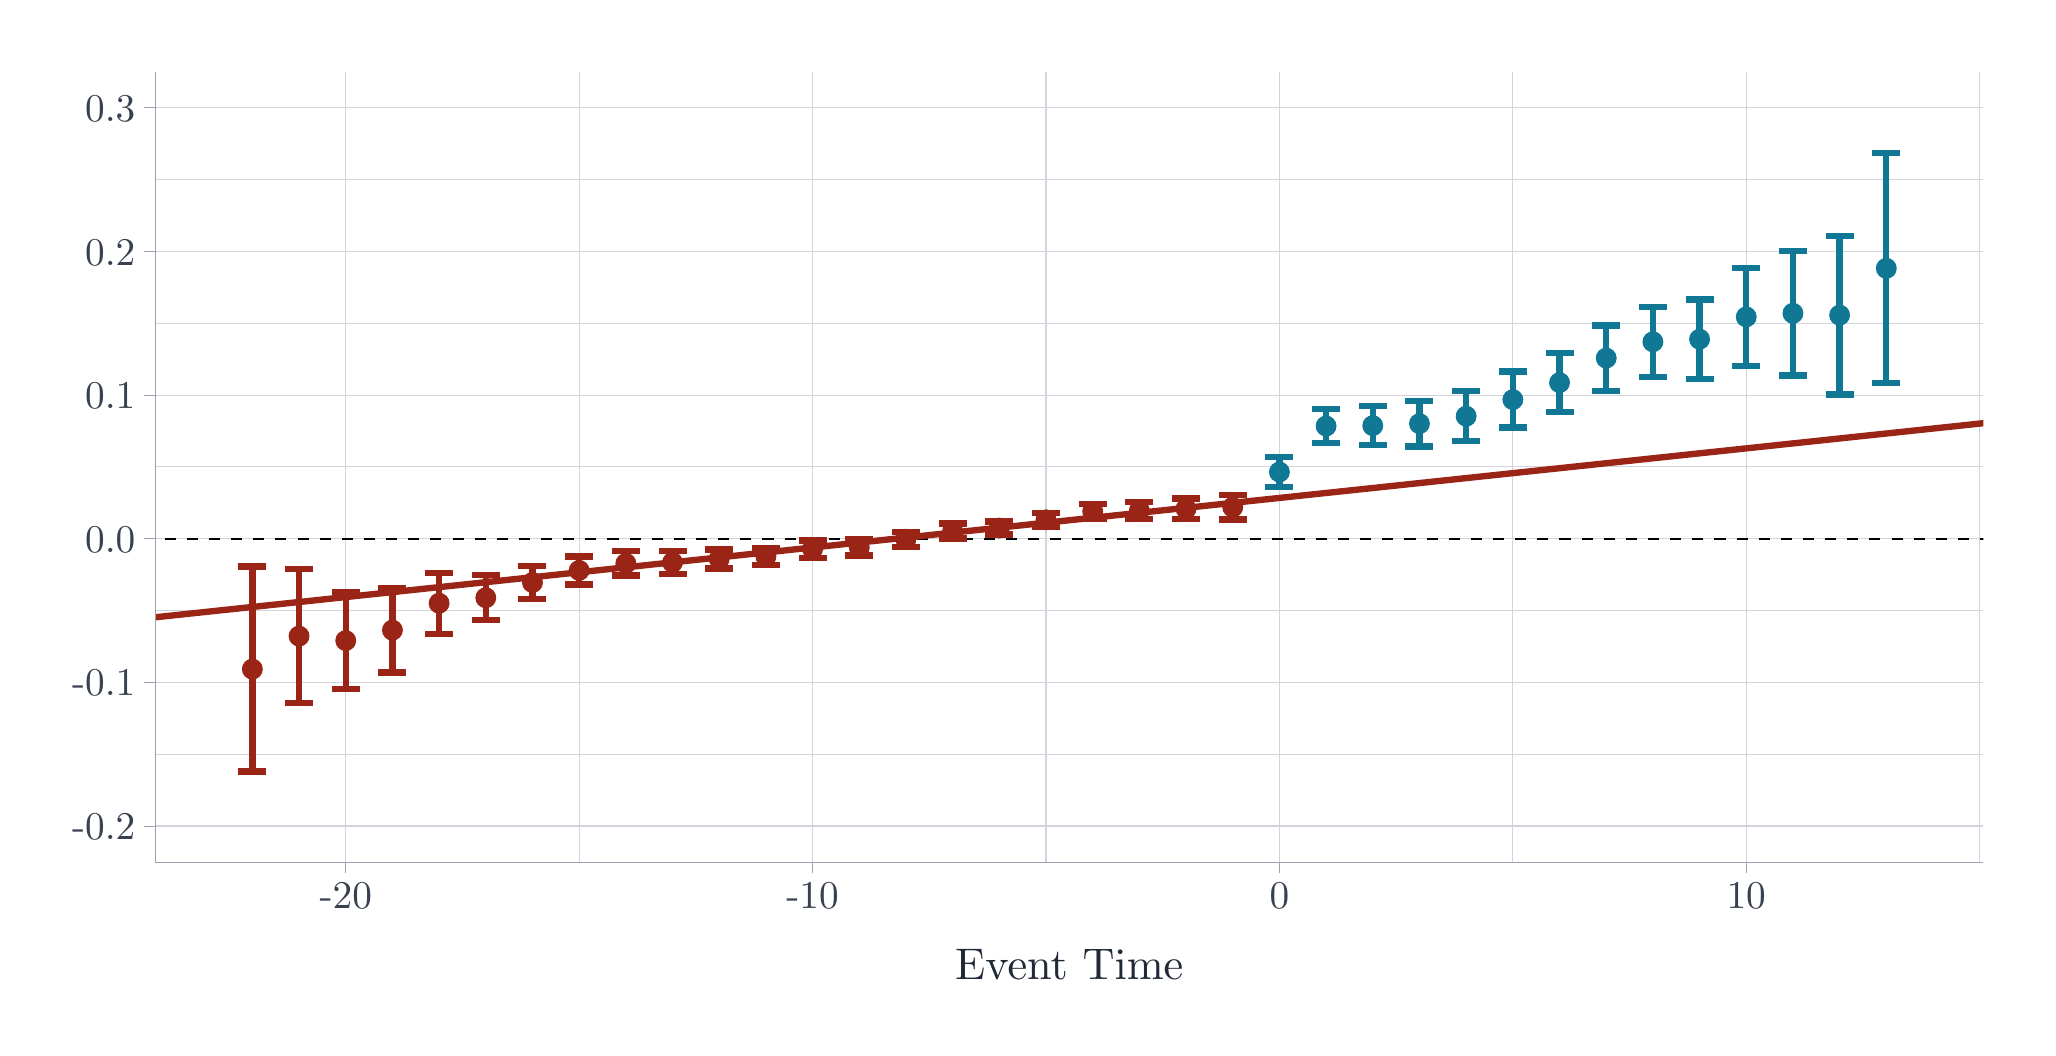
\begin{tikzpicture}[x=1pt,y=1pt]
\definecolor{fillColor}{RGB}{255,255,255}
\path[use as bounding box,fill=fillColor] (0,0) rectangle (722.70,361.35);
\begin{scope}
\path[clip] (  0.00,  0.00) rectangle (722.70,361.35);
\definecolor{drawColor}{RGB}{255,255,255}

\path[draw=drawColor,line width= 0.8pt,line join=round,line cap=round,fill=fillColor] (  0.00,  0.00) rectangle (722.70,361.35);
\end{scope}
\begin{scope}
\path[clip] ( 46.10, 59.89) rectangle (706.70,345.35);
\definecolor{drawColor}{RGB}{255,255,255}
\definecolor{fillColor}{RGB}{255,255,255}

\path[draw=drawColor,line width= 0.8pt,line join=round,line cap=round,fill=fillColor] ( 46.10, 59.89) rectangle (706.70,345.35);
\definecolor{drawColor}{RGB}{209,213,219}

\path[draw=drawColor,line width= 0.4pt,line join=round] ( 46.10, 98.81) --
	(706.70, 98.81);

\path[draw=drawColor,line width= 0.4pt,line join=round] ( 46.10,150.72) --
	(706.70,150.72);

\path[draw=drawColor,line width= 0.4pt,line join=round] ( 46.10,202.62) --
	(706.70,202.62);

\path[draw=drawColor,line width= 0.4pt,line join=round] ( 46.10,254.52) --
	(706.70,254.52);

\path[draw=drawColor,line width= 0.4pt,line join=round] ( 46.10,306.42) --
	(706.70,306.42);

\path[draw=drawColor,line width= 0.4pt,line join=round] (199.28, 59.89) --
	(199.28,345.35);

\path[draw=drawColor,line width= 0.4pt,line join=round] (367.97, 59.89) --
	(367.97,345.35);

\path[draw=drawColor,line width= 0.4pt,line join=round] (536.66, 59.89) --
	(536.66,345.35);

\path[draw=drawColor,line width= 0.4pt,line join=round] (705.35, 59.89) --
	(705.35,345.35);

\path[draw=drawColor,line width= 0.4pt,line join=round] ( 46.10, 72.86) --
	(706.70, 72.86);

\path[draw=drawColor,line width= 0.4pt,line join=round] ( 46.10,124.77) --
	(706.70,124.77);

\path[draw=drawColor,line width= 0.4pt,line join=round] ( 46.10,176.67) --
	(706.70,176.67);

\path[draw=drawColor,line width= 0.4pt,line join=round] ( 46.10,228.57) --
	(706.70,228.57);

\path[draw=drawColor,line width= 0.4pt,line join=round] ( 46.10,280.47) --
	(706.70,280.47);

\path[draw=drawColor,line width= 0.4pt,line join=round] ( 46.10,332.37) --
	(706.70,332.37);

\path[draw=drawColor,line width= 0.4pt,line join=round] (114.93, 59.89) --
	(114.93,345.35);

\path[draw=drawColor,line width= 0.4pt,line join=round] (283.62, 59.89) --
	(283.62,345.35);

\path[draw=drawColor,line width= 0.4pt,line join=round] (452.31, 59.89) --
	(452.31,345.35);

\path[draw=drawColor,line width= 0.4pt,line join=round] (621.00, 59.89) --
	(621.00,345.35);
\definecolor{drawColor}{RGB}{0,0,0}

\path[draw=drawColor,line width= 0.9pt,dash pattern=on 4pt off 4pt ,line join=round] (-614.49,176.67) -- (1367.30,176.67);
\definecolor{drawColor}{RGB}{154,36,21}

\path[draw=drawColor,line width= 2.3pt,line join=round] (-614.49, 78.16) -- (1367.30,288.56);
\definecolor{fillColor}{RGB}{154,36,21}

\path[draw=drawColor,line width= 0.4pt,line join=round,line cap=round,fill=fillColor] ( 81.19,129.56) circle (  3.57);

\path[draw=drawColor,line width= 0.4pt,line join=round,line cap=round,fill=fillColor] ( 98.06,141.49) circle (  3.57);

\path[draw=drawColor,line width= 0.4pt,line join=round,line cap=round,fill=fillColor] (114.93,139.87) circle (  3.57);

\path[draw=drawColor,line width= 0.4pt,line join=round,line cap=round,fill=fillColor] (131.80,143.65) circle (  3.57);

\path[draw=drawColor,line width= 0.4pt,line join=round,line cap=round,fill=fillColor] (148.67,153.37) circle (  3.57);

\path[draw=drawColor,line width= 0.4pt,line join=round,line cap=round,fill=fillColor] (165.54,155.35) circle (  3.57);

\path[draw=drawColor,line width= 0.4pt,line join=round,line cap=round,fill=fillColor] (182.41,160.86) circle (  3.57);

\path[draw=drawColor,line width= 0.4pt,line join=round,line cap=round,fill=fillColor] (199.28,165.24) circle (  3.57);

\path[draw=drawColor,line width= 0.4pt,line join=round,line cap=round,fill=fillColor] (216.15,167.77) circle (  3.57);

\path[draw=drawColor,line width= 0.4pt,line join=round,line cap=round,fill=fillColor] (233.01,168.11) circle (  3.57);

\path[draw=drawColor,line width= 0.4pt,line join=round,line cap=round,fill=fillColor] (249.88,169.41) circle (  3.57);

\path[draw=drawColor,line width= 0.4pt,line join=round,line cap=round,fill=fillColor] (266.75,170.27) circle (  3.57);

\path[draw=drawColor,line width= 0.4pt,line join=round,line cap=round,fill=fillColor] (283.62,172.93) circle (  3.57);

\path[draw=drawColor,line width= 0.4pt,line join=round,line cap=round,fill=fillColor] (300.49,173.59) circle (  3.57);

\path[draw=drawColor,line width= 0.4pt,line join=round,line cap=round,fill=fillColor] (317.36,176.49) circle (  3.57);

\path[draw=drawColor,line width= 0.4pt,line join=round,line cap=round,fill=fillColor] (334.23,179.47) circle (  3.57);

\path[draw=drawColor,line width= 0.4pt,line join=round,line cap=round,fill=fillColor] (351.10,180.54) circle (  3.57);

\path[draw=drawColor,line width= 0.4pt,line join=round,line cap=round,fill=fillColor] (367.97,183.51) circle (  3.57);

\path[draw=drawColor,line width= 0.4pt,line join=round,line cap=round,fill=fillColor] (384.84,186.56) circle (  3.57);

\path[draw=drawColor,line width= 0.4pt,line join=round,line cap=round,fill=fillColor] (401.71,186.87) circle (  3.57);

\path[draw=drawColor,line width= 0.4pt,line join=round,line cap=round,fill=fillColor] (418.58,187.51) circle (  3.57);

\path[draw=drawColor,line width= 0.4pt,line join=round,line cap=round,fill=fillColor] (435.44,188.06) circle (  3.57);
\definecolor{drawColor}{RGB}{16,120,149}
\definecolor{fillColor}{RGB}{16,120,149}

\path[draw=drawColor,line width= 0.4pt,line join=round,line cap=round,fill=fillColor] (452.31,200.78) circle (  3.57);

\path[draw=drawColor,line width= 0.4pt,line join=round,line cap=round,fill=fillColor] (469.18,217.40) circle (  3.57);

\path[draw=drawColor,line width= 0.4pt,line join=round,line cap=round,fill=fillColor] (486.05,217.54) circle (  3.57);

\path[draw=drawColor,line width= 0.4pt,line join=round,line cap=round,fill=fillColor] (502.92,218.27) circle (  3.57);

\path[draw=drawColor,line width= 0.4pt,line join=round,line cap=round,fill=fillColor] (519.79,220.96) circle (  3.57);

\path[draw=drawColor,line width= 0.4pt,line join=round,line cap=round,fill=fillColor] (536.66,226.94) circle (  3.57);

\path[draw=drawColor,line width= 0.4pt,line join=round,line cap=round,fill=fillColor] (553.53,233.09) circle (  3.57);

\path[draw=drawColor,line width= 0.4pt,line join=round,line cap=round,fill=fillColor] (570.40,241.96) circle (  3.57);

\path[draw=drawColor,line width= 0.4pt,line join=round,line cap=round,fill=fillColor] (587.27,247.83) circle (  3.57);

\path[draw=drawColor,line width= 0.4pt,line join=round,line cap=round,fill=fillColor] (604.14,248.78) circle (  3.57);

\path[draw=drawColor,line width= 0.4pt,line join=round,line cap=round,fill=fillColor] (621.00,256.83) circle (  3.57);

\path[draw=drawColor,line width= 0.4pt,line join=round,line cap=round,fill=fillColor] (637.87,258.15) circle (  3.57);

\path[draw=drawColor,line width= 0.4pt,line join=round,line cap=round,fill=fillColor] (654.74,257.48) circle (  3.57);

\path[draw=drawColor,line width= 0.4pt,line join=round,line cap=round,fill=fillColor] (671.61,274.39) circle (  3.57);
\definecolor{drawColor}{RGB}{154,36,21}

\path[draw=drawColor,line width= 2.3pt,line join=round] ( 76.13,166.61) --
	( 86.25,166.61);

\path[draw=drawColor,line width= 2.3pt,line join=round] ( 81.19,166.61) --
	( 81.19, 92.52);

\path[draw=drawColor,line width= 2.3pt,line join=round] ( 76.13, 92.52) --
	( 86.25, 92.52);

\path[draw=drawColor,line width= 2.3pt,line join=round] ( 93.00,165.77) --
	(103.12,165.77);

\path[draw=drawColor,line width= 2.3pt,line join=round] ( 98.06,165.77) --
	( 98.06,117.21);

\path[draw=drawColor,line width= 2.3pt,line join=round] ( 93.00,117.21) --
	(103.12,117.21);

\path[draw=drawColor,line width= 2.3pt,line join=round] (109.87,157.34) --
	(119.99,157.34);

\path[draw=drawColor,line width= 2.3pt,line join=round] (114.93,157.34) --
	(114.93,122.39);

\path[draw=drawColor,line width= 2.3pt,line join=round] (109.87,122.39) --
	(119.99,122.39);

\path[draw=drawColor,line width= 2.3pt,line join=round] (126.74,158.97) --
	(136.86,158.97);

\path[draw=drawColor,line width= 2.3pt,line join=round] (131.80,158.97) --
	(131.80,128.33);

\path[draw=drawColor,line width= 2.3pt,line join=round] (126.74,128.33) --
	(136.86,128.33);

\path[draw=drawColor,line width= 2.3pt,line join=round] (143.61,164.38) --
	(153.73,164.38);

\path[draw=drawColor,line width= 2.3pt,line join=round] (148.67,164.38) --
	(148.67,142.36);

\path[draw=drawColor,line width= 2.3pt,line join=round] (143.61,142.36) --
	(153.73,142.36);

\path[draw=drawColor,line width= 2.3pt,line join=round] (160.48,163.46) --
	(170.60,163.46);

\path[draw=drawColor,line width= 2.3pt,line join=round] (165.54,163.46) --
	(165.54,147.24);

\path[draw=drawColor,line width= 2.3pt,line join=round] (160.48,147.24) --
	(170.60,147.24);

\path[draw=drawColor,line width= 2.3pt,line join=round] (177.35,166.92) --
	(187.47,166.92);

\path[draw=drawColor,line width= 2.3pt,line join=round] (182.41,166.92) --
	(182.41,154.80);

\path[draw=drawColor,line width= 2.3pt,line join=round] (177.35,154.80) --
	(187.47,154.80);

\path[draw=drawColor,line width= 2.3pt,line join=round] (194.22,170.31) --
	(204.34,170.31);

\path[draw=drawColor,line width= 2.3pt,line join=round] (199.28,170.31) --
	(199.28,160.16);

\path[draw=drawColor,line width= 2.3pt,line join=round] (194.22,160.16) --
	(204.34,160.16);

\path[draw=drawColor,line width= 2.3pt,line join=round] (211.08,172.18) --
	(221.21,172.18);

\path[draw=drawColor,line width= 2.3pt,line join=round] (216.15,172.18) --
	(216.15,163.36);

\path[draw=drawColor,line width= 2.3pt,line join=round] (211.08,163.36) --
	(221.21,163.36);

\path[draw=drawColor,line width= 2.3pt,line join=round] (227.95,172.21) --
	(238.08,172.21);

\path[draw=drawColor,line width= 2.3pt,line join=round] (233.01,172.21) --
	(233.01,164.00);

\path[draw=drawColor,line width= 2.3pt,line join=round] (227.95,164.00) --
	(238.08,164.00);

\path[draw=drawColor,line width= 2.3pt,line join=round] (244.82,172.85) --
	(254.94,172.85);

\path[draw=drawColor,line width= 2.3pt,line join=round] (249.88,172.85) --
	(249.88,165.97);

\path[draw=drawColor,line width= 2.3pt,line join=round] (244.82,165.97) --
	(254.94,165.97);

\path[draw=drawColor,line width= 2.3pt,line join=round] (261.69,173.39) --
	(271.81,173.39);

\path[draw=drawColor,line width= 2.3pt,line join=round] (266.75,173.39) --
	(266.75,167.15);

\path[draw=drawColor,line width= 2.3pt,line join=round] (261.69,167.15) --
	(271.81,167.15);

\path[draw=drawColor,line width= 2.3pt,line join=round] (278.56,176.06) --
	(288.68,176.06);

\path[draw=drawColor,line width= 2.3pt,line join=round] (283.62,176.06) --
	(283.62,169.80);

\path[draw=drawColor,line width= 2.3pt,line join=round] (278.56,169.80) --
	(288.68,169.80);

\path[draw=drawColor,line width= 2.3pt,line join=round] (295.43,176.56) --
	(305.55,176.56);

\path[draw=drawColor,line width= 2.3pt,line join=round] (300.49,176.56) --
	(300.49,170.63);

\path[draw=drawColor,line width= 2.3pt,line join=round] (295.43,170.63) --
	(305.55,170.63);

\path[draw=drawColor,line width= 2.3pt,line join=round] (312.30,179.22) --
	(322.42,179.22);

\path[draw=drawColor,line width= 2.3pt,line join=round] (317.36,179.22) --
	(317.36,173.76);

\path[draw=drawColor,line width= 2.3pt,line join=round] (312.30,173.76) --
	(322.42,173.76);

\path[draw=drawColor,line width= 2.3pt,line join=round] (329.17,182.12) --
	(339.29,182.12);

\path[draw=drawColor,line width= 2.3pt,line join=round] (334.23,182.12) --
	(334.23,176.82);

\path[draw=drawColor,line width= 2.3pt,line join=round] (329.17,176.82) --
	(339.29,176.82);

\path[draw=drawColor,line width= 2.3pt,line join=round] (346.04,182.92) --
	(356.16,182.92);

\path[draw=drawColor,line width= 2.3pt,line join=round] (351.10,182.92) --
	(351.10,178.16);

\path[draw=drawColor,line width= 2.3pt,line join=round] (346.04,178.16) --
	(356.16,178.16);

\path[draw=drawColor,line width= 2.3pt,line join=round] (362.91,185.94) --
	(373.03,185.94);

\path[draw=drawColor,line width= 2.3pt,line join=round] (367.97,185.94) --
	(367.97,181.09);

\path[draw=drawColor,line width= 2.3pt,line join=round] (362.91,181.09) --
	(373.03,181.09);

\path[draw=drawColor,line width= 2.3pt,line join=round] (379.78,189.25) --
	(389.90,189.25);

\path[draw=drawColor,line width= 2.3pt,line join=round] (384.84,189.25) --
	(384.84,183.87);

\path[draw=drawColor,line width= 2.3pt,line join=round] (379.78,183.87) --
	(389.90,183.87);

\path[draw=drawColor,line width= 2.3pt,line join=round] (396.65,189.88) --
	(406.77,189.88);

\path[draw=drawColor,line width= 2.3pt,line join=round] (401.71,189.88) --
	(401.71,183.86);

\path[draw=drawColor,line width= 2.3pt,line join=round] (396.65,183.86) --
	(406.77,183.86);

\path[draw=drawColor,line width= 2.3pt,line join=round] (413.51,191.15) --
	(423.64,191.15);

\path[draw=drawColor,line width= 2.3pt,line join=round] (418.58,191.15) --
	(418.58,183.87);

\path[draw=drawColor,line width= 2.3pt,line join=round] (413.51,183.87) --
	(423.64,183.87);

\path[draw=drawColor,line width= 2.3pt,line join=round] (430.38,192.50) --
	(440.50,192.50);

\path[draw=drawColor,line width= 2.3pt,line join=round] (435.44,192.50) --
	(435.44,183.62);

\path[draw=drawColor,line width= 2.3pt,line join=round] (430.38,183.62) --
	(440.50,183.62);
\definecolor{drawColor}{RGB}{16,120,149}

\path[draw=drawColor,line width= 2.3pt,line join=round] (447.25,206.17) --
	(457.37,206.17);

\path[draw=drawColor,line width= 2.3pt,line join=round] (452.31,206.17) --
	(452.31,195.40);

\path[draw=drawColor,line width= 2.3pt,line join=round] (447.25,195.40) --
	(457.37,195.40);

\path[draw=drawColor,line width= 2.3pt,line join=round] (464.12,223.62) --
	(474.24,223.62);

\path[draw=drawColor,line width= 2.3pt,line join=round] (469.18,223.62) --
	(469.18,211.19);

\path[draw=drawColor,line width= 2.3pt,line join=round] (464.12,211.19) --
	(474.24,211.19);

\path[draw=drawColor,line width= 2.3pt,line join=round] (480.99,224.63) --
	(491.11,224.63);

\path[draw=drawColor,line width= 2.3pt,line join=round] (486.05,224.63) --
	(486.05,210.45);

\path[draw=drawColor,line width= 2.3pt,line join=round] (480.99,210.45) --
	(491.11,210.45);

\path[draw=drawColor,line width= 2.3pt,line join=round] (497.86,226.51) --
	(507.98,226.51);

\path[draw=drawColor,line width= 2.3pt,line join=round] (502.92,226.51) --
	(502.92,210.04);

\path[draw=drawColor,line width= 2.3pt,line join=round] (497.86,210.04) --
	(507.98,210.04);

\path[draw=drawColor,line width= 2.3pt,line join=round] (514.73,229.95) --
	(524.85,229.95);

\path[draw=drawColor,line width= 2.3pt,line join=round] (519.79,229.95) --
	(519.79,211.96);

\path[draw=drawColor,line width= 2.3pt,line join=round] (514.73,211.96) --
	(524.85,211.96);

\path[draw=drawColor,line width= 2.3pt,line join=round] (531.60,237.04) --
	(541.72,237.04);

\path[draw=drawColor,line width= 2.3pt,line join=round] (536.66,237.04) --
	(536.66,216.84);

\path[draw=drawColor,line width= 2.3pt,line join=round] (531.60,216.84) --
	(541.72,216.84);

\path[draw=drawColor,line width= 2.3pt,line join=round] (548.47,243.79) --
	(558.59,243.79);

\path[draw=drawColor,line width= 2.3pt,line join=round] (553.53,243.79) --
	(553.53,222.39);

\path[draw=drawColor,line width= 2.3pt,line join=round] (548.47,222.39) --
	(558.59,222.39);

\path[draw=drawColor,line width= 2.3pt,line join=round] (565.34,253.78) --
	(575.46,253.78);

\path[draw=drawColor,line width= 2.3pt,line join=round] (570.40,253.78) --
	(570.40,230.14);

\path[draw=drawColor,line width= 2.3pt,line join=round] (565.34,230.14) --
	(575.46,230.14);

\path[draw=drawColor,line width= 2.3pt,line join=round] (582.21,260.49) --
	(592.33,260.49);

\path[draw=drawColor,line width= 2.3pt,line join=round] (587.27,260.49) --
	(587.27,235.16);

\path[draw=drawColor,line width= 2.3pt,line join=round] (582.21,235.16) --
	(592.33,235.16);

\path[draw=drawColor,line width= 2.3pt,line join=round] (599.07,263.09) --
	(609.20,263.09);

\path[draw=drawColor,line width= 2.3pt,line join=round] (604.14,263.09) --
	(604.14,234.48);

\path[draw=drawColor,line width= 2.3pt,line join=round] (599.07,234.48) --
	(609.20,234.48);

\path[draw=drawColor,line width= 2.3pt,line join=round] (615.94,274.51) --
	(626.07,274.51);

\path[draw=drawColor,line width= 2.3pt,line join=round] (621.00,274.51) --
	(621.00,239.16);

\path[draw=drawColor,line width= 2.3pt,line join=round] (615.94,239.16) --
	(626.07,239.16);

\path[draw=drawColor,line width= 2.3pt,line join=round] (632.81,280.59) --
	(642.93,280.59);

\path[draw=drawColor,line width= 2.3pt,line join=round] (637.87,280.59) --
	(637.87,235.72);

\path[draw=drawColor,line width= 2.3pt,line join=round] (632.81,235.72) --
	(642.93,235.72);

\path[draw=drawColor,line width= 2.3pt,line join=round] (649.68,286.14) --
	(659.80,286.14);

\path[draw=drawColor,line width= 2.3pt,line join=round] (654.74,286.14) --
	(654.74,228.82);

\path[draw=drawColor,line width= 2.3pt,line join=round] (649.68,228.82) --
	(659.80,228.82);

\path[draw=drawColor,line width= 2.3pt,line join=round] (666.55,315.95) --
	(676.67,315.95);

\path[draw=drawColor,line width= 2.3pt,line join=round] (671.61,315.95) --
	(671.61,232.84);

\path[draw=drawColor,line width= 2.3pt,line join=round] (666.55,232.84) --
	(676.67,232.84);
\end{scope}
\begin{scope}
\path[clip] (  0.00,  0.00) rectangle (722.70,361.35);
\definecolor{drawColor}{RGB}{156,163,175}

\path[draw=drawColor,line width= 0.3pt,line join=round] ( 46.10, 59.89) --
	( 46.10,345.35);
\end{scope}
\begin{scope}
\path[clip] (  0.00,  0.00) rectangle (722.70,361.35);
\definecolor{drawColor}{RGB}{55,65,81}

\node[text=drawColor,anchor=base east,inner sep=0pt, outer sep=0pt, scale=  1.42] at ( 38.90, 67.97) {-0.2};

\node[text=drawColor,anchor=base east,inner sep=0pt, outer sep=0pt, scale=  1.42] at ( 38.90,119.87) {-0.1};

\node[text=drawColor,anchor=base east,inner sep=0pt, outer sep=0pt, scale=  1.42] at ( 38.90,171.77) {0.0};

\node[text=drawColor,anchor=base east,inner sep=0pt, outer sep=0pt, scale=  1.42] at ( 38.90,223.67) {0.1};

\node[text=drawColor,anchor=base east,inner sep=0pt, outer sep=0pt, scale=  1.42] at ( 38.90,275.58) {0.2};

\node[text=drawColor,anchor=base east,inner sep=0pt, outer sep=0pt, scale=  1.42] at ( 38.90,327.48) {0.3};
\end{scope}
\begin{scope}
\path[clip] (  0.00,  0.00) rectangle (722.70,361.35);
\definecolor{drawColor}{RGB}{156,163,175}

\path[draw=drawColor,line width= 0.3pt,line join=round] ( 42.10, 72.86) --
	( 46.10, 72.86);

\path[draw=drawColor,line width= 0.3pt,line join=round] ( 42.10,124.77) --
	( 46.10,124.77);

\path[draw=drawColor,line width= 0.3pt,line join=round] ( 42.10,176.67) --
	( 46.10,176.67);

\path[draw=drawColor,line width= 0.3pt,line join=round] ( 42.10,228.57) --
	( 46.10,228.57);

\path[draw=drawColor,line width= 0.3pt,line join=round] ( 42.10,280.47) --
	( 46.10,280.47);

\path[draw=drawColor,line width= 0.3pt,line join=round] ( 42.10,332.37) --
	( 46.10,332.37);
\end{scope}
\begin{scope}
\path[clip] (  0.00,  0.00) rectangle (722.70,361.35);
\definecolor{drawColor}{RGB}{156,163,175}

\path[draw=drawColor,line width= 0.3pt,line join=round] ( 46.10, 59.89) --
	(706.70, 59.89);
\end{scope}
\begin{scope}
\path[clip] (  0.00,  0.00) rectangle (722.70,361.35);
\definecolor{drawColor}{RGB}{156,163,175}

\path[draw=drawColor,line width= 0.3pt,line join=round] (114.93, 55.89) --
	(114.93, 59.89);

\path[draw=drawColor,line width= 0.3pt,line join=round] (283.62, 55.89) --
	(283.62, 59.89);

\path[draw=drawColor,line width= 0.3pt,line join=round] (452.31, 55.89) --
	(452.31, 59.89);

\path[draw=drawColor,line width= 0.3pt,line join=round] (621.00, 55.89) --
	(621.00, 59.89);
\end{scope}
\begin{scope}
\path[clip] (  0.00,  0.00) rectangle (722.70,361.35);
\definecolor{drawColor}{RGB}{55,65,81}

\node[text=drawColor,anchor=base,inner sep=0pt, outer sep=0pt, scale=  1.42] at (114.93, 42.89) {-20};

\node[text=drawColor,anchor=base,inner sep=0pt, outer sep=0pt, scale=  1.42] at (283.62, 42.89) {-10};

\node[text=drawColor,anchor=base,inner sep=0pt, outer sep=0pt, scale=  1.42] at (452.31, 42.89) {0};

\node[text=drawColor,anchor=base,inner sep=0pt, outer sep=0pt, scale=  1.42] at (621.00, 42.89) {10};
\end{scope}
\begin{scope}
\path[clip] (  0.00,  0.00) rectangle (722.70,361.35);
\definecolor{drawColor}{RGB}{31,41,55}

\node[text=drawColor,anchor=base,inner sep=0pt, outer sep=0pt, scale=  1.60] at (376.40, 17.56) {Event Time};
\end{scope}
\end{tikzpicture}
